% Options for packages loaded elsewhere
\PassOptionsToPackage{unicode}{hyperref}
\PassOptionsToPackage{hyphens}{url}
%
\documentclass[
  12pt,
]{article}
\usepackage{amsmath,amssymb}
\usepackage{iftex}
\ifPDFTeX
  \usepackage[T1]{fontenc}
  \usepackage[utf8]{inputenc}
  \usepackage{textcomp} % provide euro and other symbols
\else % if luatex or xetex
  \usepackage{unicode-math} % this also loads fontspec
  \defaultfontfeatures{Scale=MatchLowercase}
  \defaultfontfeatures[\rmfamily]{Ligatures=TeX,Scale=1}
\fi
\usepackage{lmodern}
\ifPDFTeX\else
  % xetex/luatex font selection
\fi
% Use upquote if available, for straight quotes in verbatim environments
\IfFileExists{upquote.sty}{\usepackage{upquote}}{}
\IfFileExists{microtype.sty}{% use microtype if available
  \usepackage[]{microtype}
  \UseMicrotypeSet[protrusion]{basicmath} % disable protrusion for tt fonts
}{}
\makeatletter
\@ifundefined{KOMAClassName}{% if non-KOMA class
  \IfFileExists{parskip.sty}{%
    \usepackage{parskip}
  }{% else
    \setlength{\parindent}{0pt}
    \setlength{\parskip}{6pt plus 2pt minus 1pt}}
}{% if KOMA class
  \KOMAoptions{parskip=half}}
\makeatother
\usepackage{xcolor}
\usepackage[margin=1in]{geometry}
\usepackage{graphicx}
\makeatletter
\def\maxwidth{\ifdim\Gin@nat@width>\linewidth\linewidth\else\Gin@nat@width\fi}
\def\maxheight{\ifdim\Gin@nat@height>\textheight\textheight\else\Gin@nat@height\fi}
\makeatother
% Scale images if necessary, so that they will not overflow the page
% margins by default, and it is still possible to overwrite the defaults
% using explicit options in \includegraphics[width, height, ...]{}
\setkeys{Gin}{width=\maxwidth,height=\maxheight,keepaspectratio}
% Set default figure placement to htbp
\makeatletter
\def\fps@figure{htbp}
\makeatother
\setlength{\emergencystretch}{3em} % prevent overfull lines
\providecommand{\tightlist}{%
  \setlength{\itemsep}{0pt}\setlength{\parskip}{0pt}}
\setcounter{secnumdepth}{-\maxdimen} % remove section numbering
\usepackage{fontspec}
\setmainfont{Cambria}
\usepackage{setspace}
\setstretch{1.15}
\usepackage{titlesec}
\usepackage{booktabs}
\usepackage{longtable}
\usepackage{array}
\usepackage{multirow}
\usepackage{wrapfig}
\usepackage{float}
\usepackage{colortbl}
\usepackage{pdflscape}
\usepackage{tabu}
\usepackage{threeparttable}
\usepackage{threeparttablex}
\usepackage[normalem]{ulem}
\usepackage{makecell}
\usepackage{xcolor}
\ifLuaTeX
  \usepackage{selnolig}  % disable illegal ligatures
\fi
\IfFileExists{bookmark.sty}{\usepackage{bookmark}}{\usepackage{hyperref}}
\IfFileExists{xurl.sty}{\usepackage{xurl}}{} % add URL line breaks if available
\urlstyle{same}
\hypersetup{
  pdfauthor={Anastasia Möller, Johannes Schadt, Sylviane Verschaeve, Tine Limberg},
  hidelinks,
  pdfcreator={LaTeX via pandoc}}

\title{\Huge~\textbf{Final Report:} Proteome-wide Screen for
RNA-dependent Proteins\\
\emph{non-synchronized A549 cells}}
\author{Anastasia Möller, Johannes Schadt, Sylviane Verschaeve, Tine
Limberg}
\date{17.07.2023}

\begin{document}
\maketitle

{
\setcounter{tocdepth}{2}
\tableofcontents
}
\newpage

\hypertarget{introduction}{%
\subsection{1. Introduction}\label{introduction}}

RNA-binding proteins (RBPs) constitute one of the largest families of
proteins in the cell, with over 4000 RBPs identified to date (Gebauer
et. al,2020). In addition to the examination of proteins that directly
bind RNA, this analysis encompasses RNA-dependent proteins whose
interactome relies on RNA, even without direct binding (Caudron-Herger
et al., 2019). Unlike proteins with classical RNA-binding domains, these
proteins can engage with RNA through intrinsically disordered domains
(Corley et al., 2020). For the sake of simplicity, the term ``Rdeep''
will be used in this report to refer to both RNA-binding and
RNA-dependent proteins. These proteins play a crucial role in
controlling various aspects of RNA life, function, and efficiency,
thereby acting as essential regulators in numerous cellular processes.
Rdeeps are involved in extensive regulatory networks that govern
critical processes, including transcription, splicing, RNA modification,
intracellular trafficking, translation, and decay (Corley et al., 2020).
The significance of Rdeeps in human health is underscored by their
involvement in a wide range of diseases. Mutations in genes encoding
Rdeeps have been identified as the underlying cause of various
disorders, leading to malfunction and tissue-specific defects. Rdeeps
are particularly implicated in diseases of the nervous system and
cancers, making them promising targets for therapeutic interventions.
Remarkably, the prevalence of RBP mutations in diseases is substantial,
with nearly one-third of Rdeeps implicated in various pathologies,
encompassing over a thousand disease-related Rdeeps identified thus far.
In mendelian disorders, Rdeeps outnumber other classes of proteins,
including transcription factors, in terms of the prevalence of mutations
(Gebauer et. al,2020). To comprehensively elucidate the involvement of
Rdeeps in translational control and their roles in disease pathogenesis,
further investigations are required. Understanding the mechanistic
interplay between Rdeeps and RNA in cellular processes holds great
promise for developing targeted therapeutic strategies to rectify
RBP-related dysfunctions. Therefore, the goal of this analysis is, to
identify which proteins in the given dataset are Rdeeps. The dataset to
be analysed contains 3680 different proteins from synchronized mitotic
A549 cells. At the end of this project, a linear regression will be
developed, which will make it possible to predict RNA dependence for
proteins based on their distribution of the control and RNase treated
sample.

\hypertarget{experimental-setup}{%
\subsubsection{1.1. Experimental Setup}\label{experimental-setup}}

\renewcommand{\section}{\titlespacing*{\section}{0pt}{0.3\baselineskip}{0.2\baselineskip}\section}

To collect the mass spectrometry data, a strict protocol was followed.
The non-synchronized A549 cells were centrifuged and lysed. One sample
was treated with RNAse, while the other served as the untreated control.
Both samples were divided into 25 fractions using a sucrose gradient.
Ultracentrifugation was performed, allowing the proteins to distribute
based on their density. For statistical relevance, the protocol included
three repetitions of the experiment. Therefore, triplicates are
available for each protein for both Control and RNase. The fractions
were then subjected to mass spectrometry analysis to determine the
protein abundance, measured in arbitrary units (Caudron-Herger et al.,
2019). Furthermore, it should be noted that the protein amount is
represented by the y-value whilst the number of the fraction is the
x-value.

\hypertarget{methods}{%
\subsection{2. Methods}\label{methods}}

\hypertarget{data-cleanup}{%
\subsubsection{2.1. Data cleanup}\label{data-cleanup}}

\renewcommand{\subsection}{\titlespacing*{\subsection}{0pt}{0.3\baselineskip}{0.2\baselineskip}\subsection}

The data clean up consists of checking for missing values and if
necessary deleting rows of zeros. Furthermore, the columns are reordered
to facilitate the separation of the dataset into two dataframes one
containing Control while the other consists of the RNase group.

\hypertarget{reproducibility}{%
\subsubsection{2.2. Reproducibility}\label{reproducibility}}

\renewcommand{\section}{\titlespacing*{\section}{0pt}{0.3\baselineskip}{0.2\baselineskip}\section}

The reproducibility of the replicates (rep) for the Control and the
RNase group is calculated separately by computing the pearson
correlation between rep1 and rep2, rep1 and rep3 as well as between rep2
and rep3. There are 2 scenarios where a protein is seen as not
reproducible. Firstly, if a replicate of a protein has only zeros, its
correlation can not be calculated (NA) and the protein is discarded. 83
proteins are affected. Moreover, if all 3 correlations either in the
Control or RNase group of one protein are below 0.9 the protein isn't
reliable enough for further analysis. Thus 523 proteins are additionally
deleted, resulting 3074 proteins from initially 3680 proteins are left
for further analysis. Some proteins contain two replicates similar to
each other (correlation \textless{} 0.9) and a third one that completely
differs. Knowing that these proteins have one high and two smaller
correlations, the deviating replicate was set to NA and will be ignored
when uniting the replicates per protein. Consequently, important data is
preserved without loosing too many proteins.

\hypertarget{normalization-methods-and-reduction}{%
\subsubsection{2.3. Normalization methods and
Reduction}\label{normalization-methods-and-reduction}}

\renewcommand{\section}{\titlespacing*{\section}{0pt}{0.3\baselineskip}{0.2\baselineskip}\section}

Since each normalisation method has advantages and disadvantages, we
apply three different methods to the dataframe. The \textbf{mean-value
method (mvm)} is the first data normalisation we use. The mean protein
amount of each protein is substracted from the protein amount in each
fraction.The values that are zero or smaller than the mean become
negative through this subtraction. We set these negative values to zero
to simplify further analysis. Afterwards, the sum of the proteinamount
in each row is scaled to 100. Furthermore we used the
\textbf{z-transformation}, which transforms our data into a standard
normal distribution with a mean of 0 and a standard deviation of 1 by
using the formula: Z = (X - μ) / σ. To avoid negative values and not
lose to much information as we did with the mean-value method, the
smallest value per protein is added to each fraction of the
corresponding protein, meaning the smallest value is now 0. In case of
the z-transformation we first normalized than scaled to 100. Afterwards
we reduced by calculating the mean between the replicates with a higher
correlation than 0.9 and scaled again to 100. The last used
normalization method is \textbf{Min-Max scaling (mms)}, which is a very
simple scaling-method where the normalized value \(x'\) is calculated
from the original value \(x\) as follows:
\(x'=\frac{{x-\text{min}(x)}}{{\text{max}(x)-\text{min}(x)}}\). This
means that the highest value is automaticly set to one and the lowest
values to zero. With this method it is very easy to calculate the global
peaks, but on the other hand, the protein amount, so the area beneath
the graph cannot be normalized.

\hypertarget{gaussian-fit}{%
\subsubsection{2.4. Gaussian fit}\label{gaussian-fit}}

\renewcommand{\section}{\titlespacing*{\section}{0pt}{0.3\baselineskip}{0.2\baselineskip}\section}

Goal of the gaussian fit is to fit a gaussian function to the data
points, in our case the protein amount in each fraction of one protein.
Therefore, we establish a list in which the parameters, which describe
the distribution are saved. To fit the parameters to our data we used
the optim() function implemented in R.

\hypertarget{data-description-via-parameters}{%
\subsubsection{2.6. Data description via
Parameters}\label{data-description-via-parameters}}

\renewcommand{\section}{\titlespacing*{\section}{0pt}{0.3\baselineskip}{0.2\baselineskip}\section}

To identify whether a Protein is RNA dependent or not each protein is
tested on 4 parameters. The goal of those 4 parameters is the
identification of significant differences between the Control and RNase
sample. In the following sections the parameters will be elaborated.

\hypertarget{parameter-1-significant-change-of-protein-amount-under-global-peak}{%
\subsubsection{2.6.1. Parameter 1: Significant change of protein amount
under global
peak}\label{parameter-1-significant-change-of-protein-amount-under-global-peak}}

\renewcommand{\section}{\titlespacing*{\section}{0pt}{0.3\baselineskip}{0.2\baselineskip}\section}

The first parameter identifies a significant change of the protein
amount under the global peak for each protein. The global maximum
represents the fraction of the sucrose gradient containing the highest
protein amount. It is determined by using the \emph{which.max()}
function for each protein. If the Protein amount of the global peak
fraction is either in the Control or RNase sample 1.7 times higher than
the other sample, we defined it as a significant change.

\hypertarget{parameter-2-significant-change-of-protein-amount-under-local-peaks}{%
\subsubsection{2.6.2. Parameter 2: Significant change of protein amount
under local
peaks}\label{parameter-2-significant-change-of-protein-amount-under-local-peaks}}

\renewcommand{\section}{\titlespacing*{\section}{0pt}{0.3\baselineskip}{0.2\baselineskip}\section}

The next parameter recognizes a significant change in the total protein
amount under the local peaks between the Control and RNase sample for
each protein. New local peaks can occur if after RNase treatment the
protein either dissociates or gains new interaction partners. To detect
a significant change the local peaks have to be identified. To be
defined as a local peak four criteria have to be fulfilled. First, the
y-value of the local peak fraction has to be higher than the y-value of
its neighbor fractions. Afterwards we checked if the sd of the local
peak's y-value and its neighbors is higher than the sd of the y-values
which contain less than 8 \% of the total protein amount
(\emph{sd.threshold}). The aim is to sort out small fluctuation between
the y-values. The third criteria selects the relevant local peaks by
sorting those out which have a smaller protein amount than 3 \% of the
total protein amount. Most of the already mentioned criteria fit to the
global peaks as well and thus global maxima have to be removed. The
total protein amount under the local peaks for each protein in the
Control and RNase sample is of interest. If it differs more than 7.5
from each other a significant change of the protein amount under the
local peak is present.

\hypertarget{parameter-3-significant-fraction-shift-of-global-peak}{%
\subsubsection{2.6.3. Parameter 3: Significant fraction-shift of global
peak}\label{parameter-3-significant-fraction-shift-of-global-peak}}

\renewcommand{\section}{\titlespacing*{\section}{0pt}{0.3\baselineskip}{0.2\baselineskip}\section}

The third parameter focuses on the x-axis depicting the fractions. If
the fraction of the global peak in either the Control or RNase sample
differs more than two fractions in the positive or negative x-direction
compared to the other sample, the protein is defined as RNA-dependent.
It lost or gained an interaction partner due to the RNase treatment.

\hypertarget{parameter-4-significant-difference-in-position-of-shoulderregions}{%
\subsubsection{2.6.4. Parameter 4: Significant difference in position of
shoulderregions}\label{parameter-4-significant-difference-in-position-of-shoulderregions}}

\renewcommand{\section}{\titlespacing*{\section}{0pt}{0.3\baselineskip}{0.2\baselineskip}\section}

At last it is observed if shoulderregions occur or disappear after the
RNase treatment. A shoulderregion contains more than 2 consecutive
fractions with a sd less than the \emph{sd.threshold}. On the contrary
to the local peak identification the fractions with small fluctuations
are sorted. Of interest are those fractions belonging to shoulderregions
which either occur in the Control or RNase sample but not in both.Often
parts of the shoulderregions are overlapping, resulting in
shoulderregions of interest with less than 3 consecutive fractions. So,
a shoulderregion of interest is only significant if it has three or more
consecutive fractions.

\begin{verbatim}
## Warning: Paket 'ggplot2' wurde unter R Version 4.2.3 erstellt
\end{verbatim}

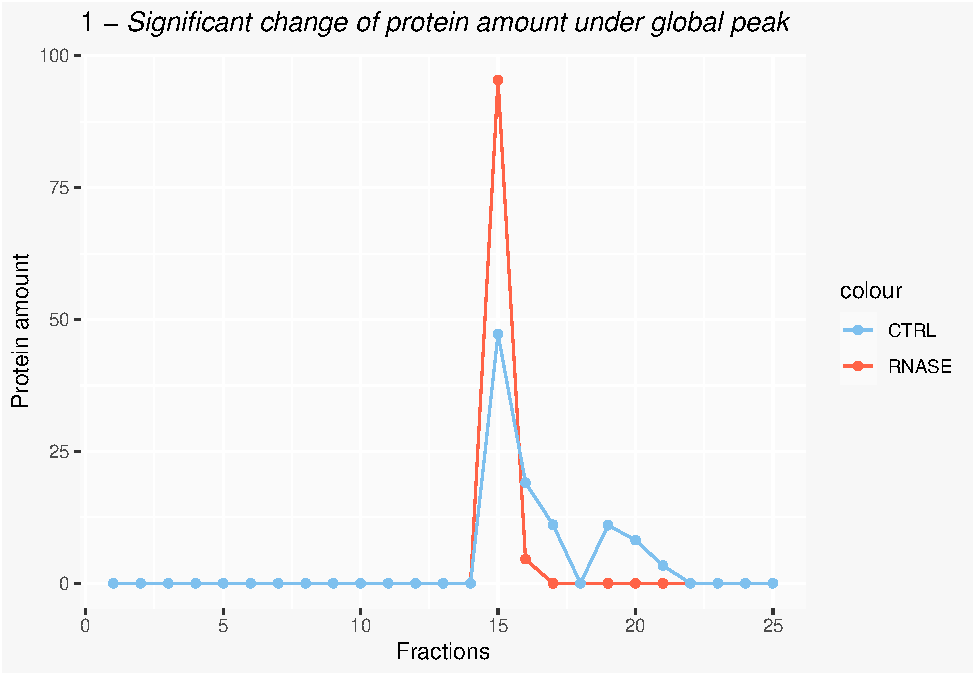
\includegraphics[width=0.45\linewidth]{final_files/figure-latex/unnamed-chunk-2-1}
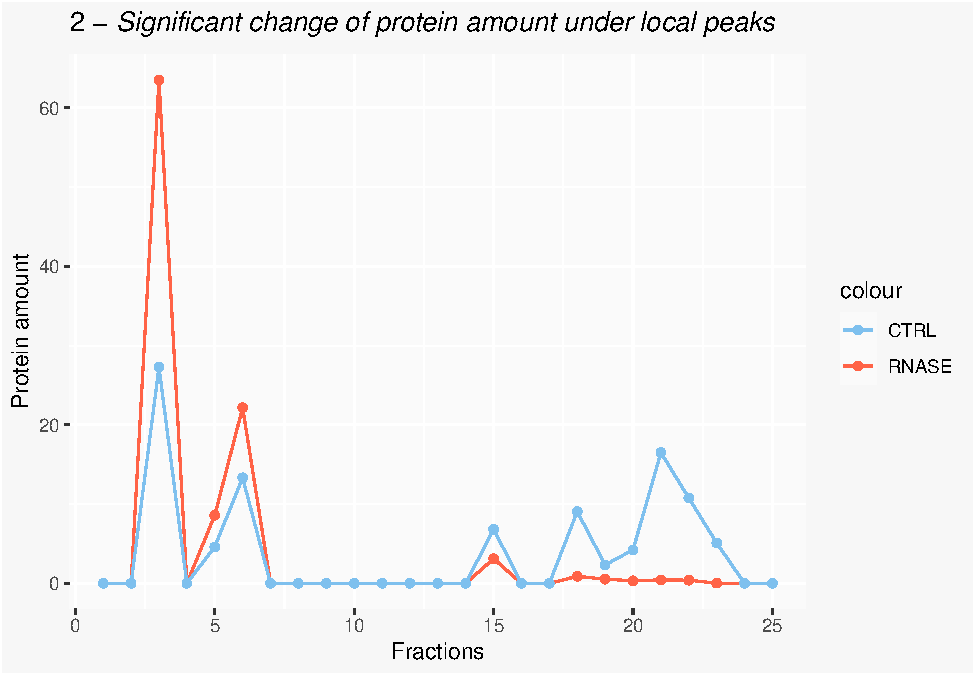
\includegraphics[width=0.45\linewidth]{final_files/figure-latex/unnamed-chunk-2-2}
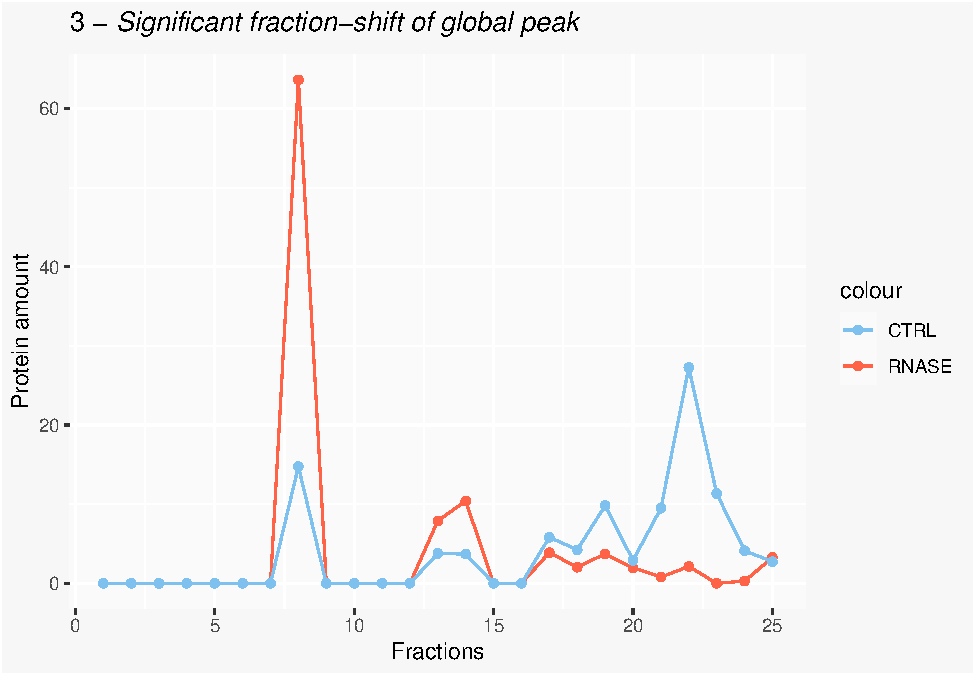
\includegraphics[width=0.45\linewidth]{final_files/figure-latex/unnamed-chunk-2-3}
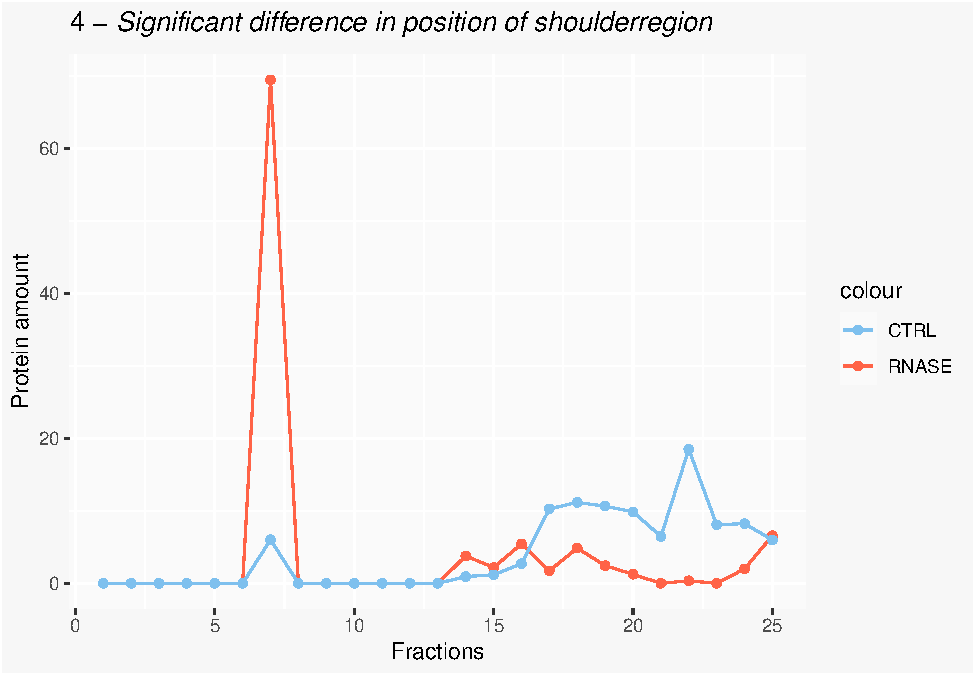
\includegraphics[width=0.45\linewidth]{final_files/figure-latex/unnamed-chunk-2-4}

\hypertarget{boundaries-and-precipitated-proteins}{%
\subsubsection{2.6.5. Boundaries and Precipitated
proteins}\label{boundaries-and-precipitated-proteins}}

The local peakfinder can't find local maxima at the boundaries (fraction
1 and fraction 25) because they have only one neighbor fraction. A local
peak at the boundary has to fulfill following requirements. Firstly, it
has to have a higher y-value than the two succeeding fractions.
Secondly, the protein amount of those three fractions has to be bigger
than 10. Smaller protein amounts are not relevant enough. Also
precipitated proteins are not described by the parameters and have to be
identified separately. They have a global peak in fraction 25 and their
total protein amount of 100 has to be split between fraction 23, 24 and
25.

\hypertarget{k-means-clustering}{%
\subsubsection{2.7. K-means clustering}\label{k-means-clustering}}

Kmeans is used to group a set of data points of a \(d\) - dimensional
space into a certain number \(k\) of clusters. Each cluster has a
center, the so called centroid. At the beginning of the clustering
process \(k\) number of clusters are set randomly. Then, the following
steps have to be repeated again and again (\(n\)-times), until no
further change can be obeserved: 1. The points are assigned to the
cluster to whose centroid they are closest to. The distance is commonly
the euclidean distance. 2. Thus, the centers of the clusters change and
the centroids move. In our case we grouped our proteins in a
two-dimensional space (fraction of control-peak and fraction of rnase)
into \(k=4\) clusters. We performed kmeans to have an alternative Method
for identification of RNA-dependent Proteins, besides our Parameters.

\hypertarget{regression-analysis}{%
\subsubsection{2.8. Regression analysis}\label{regression-analysis}}

The linear regression models the mathematical relationship between a
dependent variable and a independent variable. The linear equation is
represented as y = mx + n.~To analyse the model two values have to be
taken into account. At first if the \emph{p-value} is above 5 \%, the
model has to be discarded. Furthermore, the R-squared value describes
the model's accuracy representing the proportion of the variance in the
dependent variable that can be explained by the independent variables.
Tow regression models are generated, both working with the pearson
correlation between the Control and RNase protein amounts as the
independent variable. The two models differ in their dependent variable.
One uses the result of our four parameters, while the other uses the
global shift amount in fractions. They are trained with 80 \% of our
dataset, so a prediction can be made for the remaining 20 \%.

\hypertarget{results}{%
\subsection{3. Results}\label{results}}

\hypertarget{gaussian-fit-1}{%
\subsubsection{3.1 Gaussian fit}\label{gaussian-fit-1}}

On the grounds of our lists, containing the parameters for the gaussian
distribution for every protein, it is possible to plot the gaussian
curves. The control and RNase curves can be plotted separately or
together in one plot for better comparison. Because, we use the optim()
function and to not implement further parameters ourselves, the
distribution does not show local peaks or shoulder regions.
Therefore,the gaussian fit is only used for visualisation not for
further analysis. \textbf{Graph ???}

\hypertarget{rna-dependent-proteins}{%
\subsubsection{3.2. RNA-dependent
Proteins}\label{rna-dependent-proteins}}

Using just parameter 1 (global peaks), we were able to characterize the
shift-type, so whether the peaks show no shift, a right shift, a left
shift, or are precipitated. The graph below visualizes our results for
MVM. Using only parameter 1 we were able to identify 368 RNA-dependent
Proteins with MVM, 349 with z-transformation and 320 with MMS. Using our
parameters, we were able to identify 464 RNA-dependent proteins with
MVM, 468 with z-transformation and 396 with MMS. The following plot
shows the significance of the different parameters and how they they
contributed to the characterization for MVM. All proteins that have two
positive parameters and all proteins that have solely a global shift are
classified as RNA-dependent.

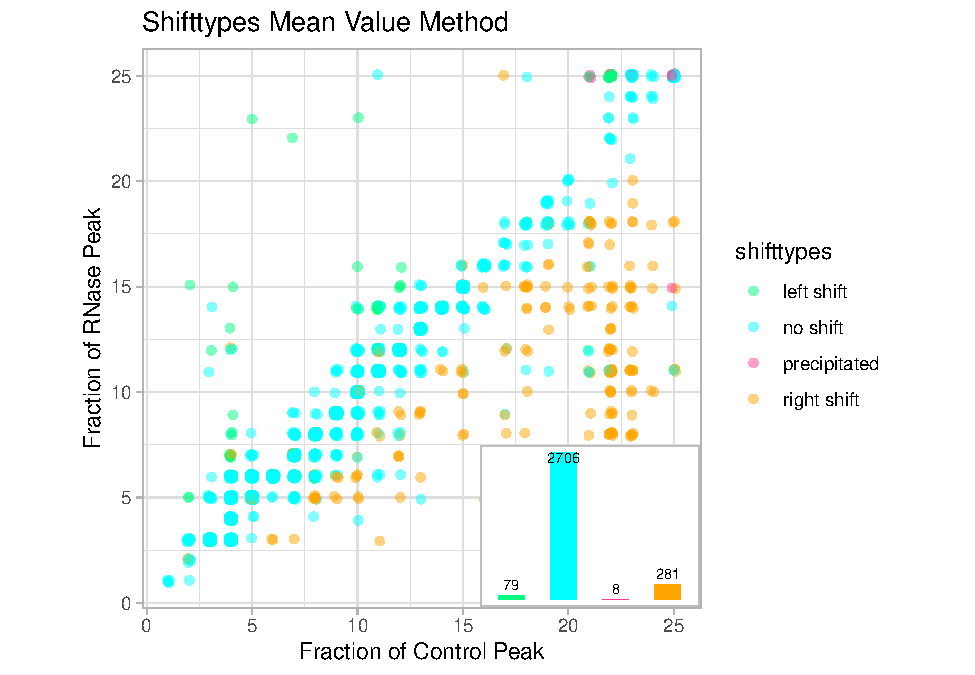
\includegraphics[width=0.5\linewidth]{final_files/figure-latex/unnamed-chunk-3-1}
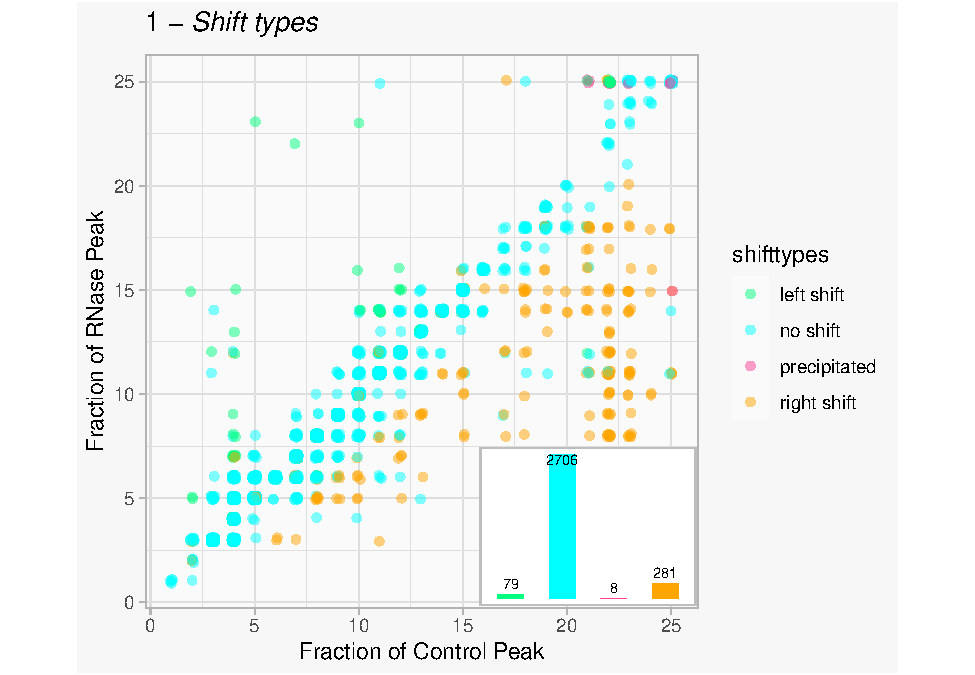
\includegraphics[width=0.5\linewidth]{final_files/figure-latex/unnamed-chunk-3-2}
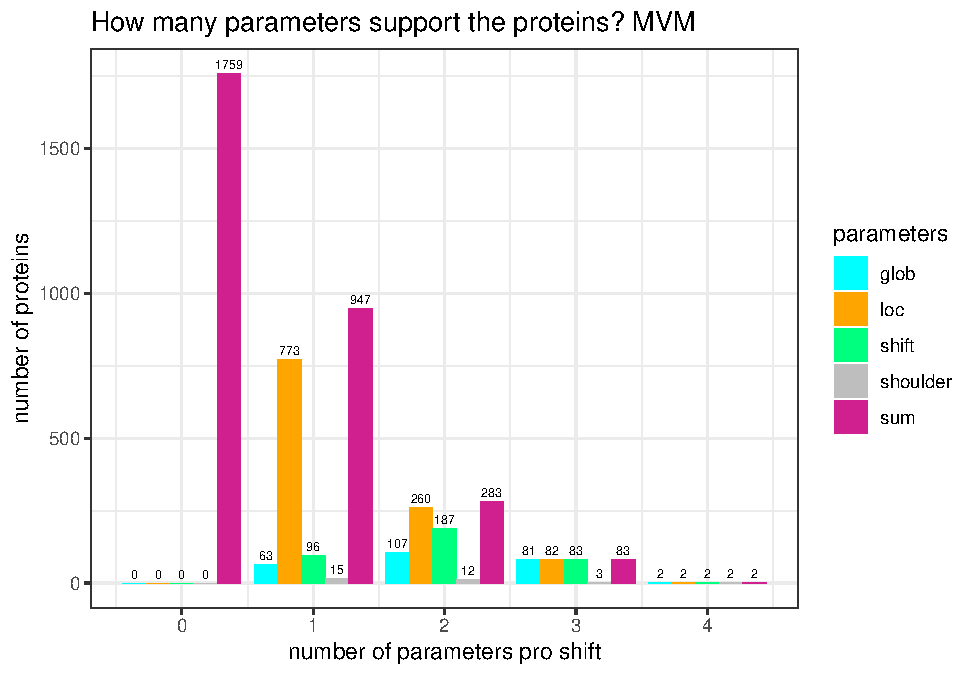
\includegraphics[width=0.5\linewidth]{final_files/figure-latex/unnamed-chunk-3-3}
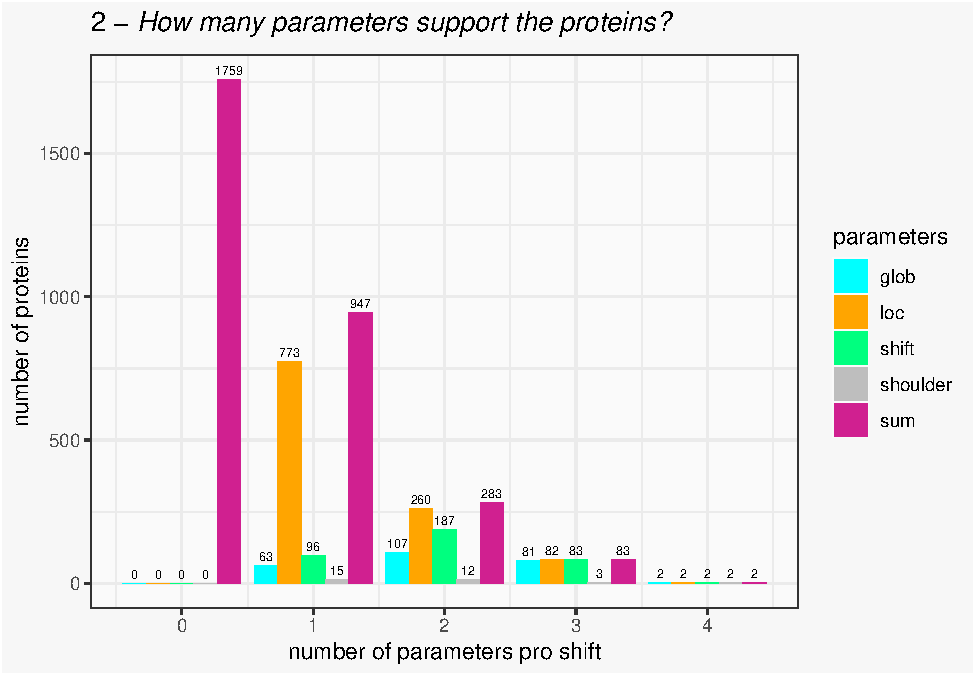
\includegraphics[width=0.5\linewidth]{final_files/figure-latex/unnamed-chunk-3-4}

\hypertarget{k-means-clustering-1}{%
\subsubsection{3.3. K-means clustering}\label{k-means-clustering-1}}

We want to cluster the Proteins depending on their global control peaks
and their global RNase Peaks. To find out how many proteins would be
optimal in theory we used the elbow method that showed us, that two
clusters would be optimal. But looking at the biological background, two
clusters would not help us to identify RNA-dependent proteins, but
rather group them into heavy and light proteins. To gain useful results
from kmeans, we forced it to create four clusters. Kmeans clustered the
proteins as followed:

We chose the cluster at the bottom right for every normalization method,
to be RNA-dependent (for MVM this would be cluster two). The other
clusters can't be identified as RNA-dependent or not. There are no
visible differences between the RNA-dependent proteins clusters of the
different normalization methods. Using kmeans we were able to identify
160 RNA-associated Proteins for MVM, 155 for z-transformation and 159
for Min-Max-Scaling.

\hypertarget{regression-analysis-1}{%
\subsubsection{3.4. Regression analysis}\label{regression-analysis-1}}

The two already described regression models show both a p-value below
0.05 and therefore they can be used for further analysis. The highest
R-squared values are detected for the z-transformed data: the model
based on the parameters shows a R-squared value of 0.43, while in the
model using the global shift amount the R-squared value is 0.66. The
model with the higher R-squared value is visualized in the plot below.
Each protein is depicted as a dot. As expected the majority of the
trained data, marked in grey shows a high correlation and a shift under
2 fractions. On the other hand those with a small correlation have a
shift upwards of 2 fractions. As already decided for the parameter
\textbf{Significant fraction-shift of global peak}: a protein is
classified as RNA-dependent protein if it has a shift higher than two
fractions. The threshold is marked as a green line in the plot.

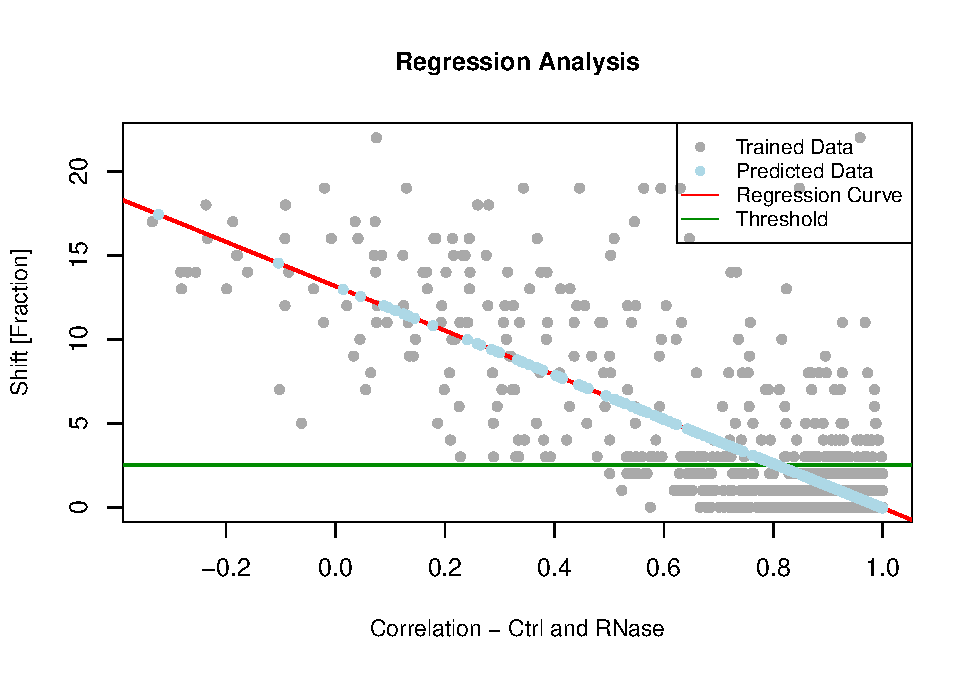
\includegraphics{final_files/figure-latex/unnamed-chunk-5-1.pdf}

\hypertarget{comparison-with-database}{%
\subsubsection{3.5. Comparison with
Database}\label{comparison-with-database}}

We compared our results with the RDeep Database and a table containing
non-RNA-associated Proteins from another paper (Quelle?). The following
table shows how well the Method via our parameters worked. The table on
the left shows the number of true positives, false positives, true
negatives and false negatives. The table on the right shows the false
negative rate (FNR), the false positive rate (FPR) and the precision.

\begin{table}
\centering
\begin{tabular}{l|r|r|r}
\hline
  & mvm & zt & mms\\
\hline
True Positives & 422 & 417 & 356\\
\hline
False Positives & 39 & 47 & 37\\
\hline
True Negatives & 695 & 687 & 697\\
\hline
False Negatives & 1905 & 1910 & 1971\\
\hline
\end{tabular}
\end{table}

\begin{table}
\centering
\begin{tabular}{l|r|r|r}
\hline
  & mvm & zt & mms\\
\hline
FNR & 0.8187 & 0.8208 & 0.8470\\
\hline
FPR & 0.0531 & 0.0640 & 0.0504\\
\hline
Precision & 0.9154 & 0.8987 & 0.9059\\
\hline
\end{tabular}
\end{table}

The following tables do the same for our kmeans results:

\begin{table}

\caption{\label{tab:unnamed-chunk-7}Tabelle 1}
\centering
\begin{tabular}[t]{l|r|r|r}
\hline
  & mvm & zt & mms\\
\hline
True Positives & 152 & 145 & 151\\
\hline
False Positives & 7 & 9 & 7\\
\hline
True Negatives & 727 & 725 & 727\\
\hline
False Negatives & 2175 & 2182 & 2176\\
\hline
\end{tabular}
\end{table}

\begin{table}
\centering
\begin{tabular}{l|r|r|r}
\hline
  & mvm & zt & mms\\
\hline
FNR & 0.9347 & 0.9377 & 0.9351\\
\hline
FPR & 0.0095 & 0.0123 & 0.0095\\
\hline
Precision & 0.9560 & 0.9416 & 0.9557\\
\hline
\end{tabular}
\end{table}

The following tables do the same for our results that only depended on
out global shift:

\begin{table}
\centering
\begin{tabular}{l|r|r|r}
\hline
  & mvm & zt & mms\\
\hline
True Positives & 339 & 315 & 336\\
\hline
False Positives & 26 & 31 & 31\\
\hline
True Negatives & 708 & 703 & 703\\
\hline
False Negatives & 1988 & 2012 & 1991\\
\hline
\end{tabular}
\end{table}

\begin{table}
\centering
\begin{tabular}{l|r|r|r}
\hline
  & mvm & zt & mms\\
\hline
FNR & 0.8543 & 0.8646 & 0.8556\\
\hline
FPR & 0.0354 & 0.0422 & 0.0422\\
\hline
Precision & 0.9288 & 0.9104 & 0.9155\\
\hline
\end{tabular}
\end{table}

There are thirteen proteins, that are not present neither in the RDeep
data set, nor the table containing non-RNA-associated Proteins from the
paper.

\hypertarget{discussion}{%
\subsection{4. Discussion}\label{discussion}}

The goal was to identify RNA-dependent proteins using the data provided
by mass-spectrometry. -\textgreater{} t-test

Regarding the regression analysis, the R-squared values differ notably.
This can be explained with the following information: for the model
based on the results of the parameters, we used zeros for non-Rdeep
proteins and ones for proteins we classified as Rdeep, resulting in a
low range and therefore a worse linear relationship. The second model
has a higher range because we used the shift amount in fractions as the
dependent variable, thus has a better linear relationship, shown by the
higher R-squared value. To find the Rdeep proteins, we used several
methods to find out which variant of our analysis was the best. Overall,
we had a very high false negative rate, independent of the methods we
used. The lowest was 81.9\%. This could be, because our criteria were to
strict (e.g.~\textbf{w}). But it has to be taken into account that the
method used in the experiment is not able to detect all RNA-dependent
proteins. The RDeep Database uses the results of many different papers
that used all sorts of different experiments to identify RNA-dependent
proteins. So it is impossible for our results to have a low
false-negative rate. (\textbf{unterschiedliche Zellstadien?}) More
important for us would be to look at the false-positive rate and
precision of our results: Through all methods, normalization via
mean-values method was the best. It led to the lowest false-negative
rates, the lowest false-positive rates and the highest precision.
z-transformation seams to have been the worst of the three methods. So,
mean-value method is the normalization method that should be used when
analyzing this sort of data. (\textbf{Why?}) The following applies to
our MVM-results, but is similar to our z-transformation results and MMS
results. If we look at the results of kmeans, our parameters and global
shift alone, we observe that kmeans is the most precise, but also leaves
out a lot more RNA-dependent proteins that were detected by other
methods.This is because, we only chose one cluster, that probably
contained right shift proteins, leaving out all precipitated and left
shifting proteins. To increase the number of proteins found this way, we
would have to create more clusters and choose them accordingly. Looking
at the false negative rate of the results of only the global shift, it
is clear that the global shift already detects more RNA-dependent
proteins than kmeans, but also has a higher false positive rate.~Still,
the low false-positive rate of our global shift results is quite low,
and validates our decision to qualify proteins that solely have a global
shift, but no other positive parameter, as RNA-dependent. If we look at
the results of our four parameters, we see the same pattern. We found
way more RNA-dependent proteins, but the false positive rate increased
as well. In summary: If we want to be sure that the proteins we identify
as RNA dependent, really are RNA dependent, we should choose kmeans. But
we have to embrace the possibility that we miss a lot of proteins. If we
want to detect many proteins, we should choose our parameters, but take
into account that our precision will go down by about 4-5\% depending on
the normalization method. Looking at the global shift as sole parameter,
would be a comprise between precision and quantity. But even with kmeans
clustering, our false positive rate is at about 1\%, so the results
should be verified by another method. Using our methods, we were able to
detect 13 new proteins that are not part of the RDeep Database, of which
1-4 are Rdeep, depending on the normalization method used. These
proteins could be analysed further with additional experiments, and be
added to RDeep.

\hypertarget{outlook}{%
\subsection{5. Outlook}\label{outlook}}

With our analysis we verified numerous Rdeeps and identified 1 to 4 new
ones. Nevertheless, for medical applications their cellular function and
potential mutations causing the proteins malfunction and leading to
diseases have to be investigated.

\hypertarget{literature}{%
\subsection{6. Literature}\label{literature}}

Gebauer et al., RNA-binding proteins in human genetic disease, 2020,
Nature Reviews Genetics

Caudron-Herger et al., R-DeeP: Proteome-wide and Quantitative
Identification of RNA-Dependent Proteins by Density Gradient
Ultracentrifugation, 2019, Molecular Cell

Corley et al., How RNA-Binding Proteins Interact with RNA: Molecules and
Mechanisms, 2020, Molecular Cell

\hypertarget{appendix}{%
\subsection{7. Appendix}\label{appendix}}

The following tables show the names of these proteins and whether they
are considered as RNA-dependent by our analysis or not. On the left side
are the results using our parameters, on the right side the ones
obtained by kmeans:

\begin{table}
\centering
\begin{tabular}{l|r|l|r|l|r}
\hline
mvm & shift? & zt & shift? & mms & shift?\\
\hline
PBIR3\_HUMAN & 0 & PBIR3\_HUMAN & 0 & PBIR3\_HUMAN & 0\\
\hline
MPP6\_HUMAN & 0 & MPP6\_HUMAN & 0 & MPP6\_HUMAN & 0\\
\hline
F207A\_HUMAN & 1 & F207A\_HUMAN & 1 & F207A\_HUMAN & 1\\
\hline
CCD58\_HUMAN & 0 & CCD58\_HUMAN & 0 & CCD58\_HUMAN & 0\\
\hline
BZW2\_HUMAN & 0 & BZW2\_HUMAN & 0 & BZW2\_HUMAN & 0\\
\hline
UBIM\_HUMAN & 1 & UBIM\_HUMAN & 1 & UBIM\_HUMAN & 1\\
\hline
ACOC\_HUMAN & 0 & ACOC\_HUMAN & 0 & ACOC\_HUMAN & 0\\
\hline
PHB\_HUMAN & 0 & PHB\_HUMAN & 0 & PHB\_HUMAN & 0\\
\hline
UTRO\_HUMAN & 0 & UTRO\_HUMAN & 0 & UTRO\_HUMAN & 0\\
\hline
RT36\_HUMAN & 1 & RT36\_HUMAN & 1 & RT36\_HUMAN & 1\\
\hline
DIEXF\_HUMAN & 0 & DIEXF\_HUMAN & 0 & DIEXF\_HUMAN & 0\\
\hline
BZW1\_HUMAN & 0 & BZW1\_HUMAN & 1 & BZW1\_HUMAN & 0\\
\hline
WDR92\_HUMAN & 0 & WDR92\_HUMAN & 0 & WDR92\_HUMAN & 0\\
\hline
13 & 3 & 13 & 4 & 13 & 3\\
\hline
\end{tabular}
\end{table}

\begin{table}
\centering
\begin{tabular}{l|r|l|r|l|r}
\hline
mvm & shift? & zt & shift? & mms & shift?\\
\hline
PBIR3\_HUMAN & 0 & PBIR3\_HUMAN & 0 & PBIR3\_HUMAN & 0\\
\hline
MPP6\_HUMAN & 0 & MPP6\_HUMAN & 0 & MPP6\_HUMAN & 0\\
\hline
F207A\_HUMAN & 0 & F207A\_HUMAN & 0 & F207A\_HUMAN & 0\\
\hline
CCD58\_HUMAN & 0 & CCD58\_HUMAN & 0 & CCD58\_HUMAN & 0\\
\hline
BZW2\_HUMAN & 0 & BZW2\_HUMAN & 0 & BZW2\_HUMAN & 0\\
\hline
UBIM\_HUMAN & 0 & UBIM\_HUMAN & 0 & UBIM\_HUMAN & 0\\
\hline
ACOC\_HUMAN & 0 & ACOC\_HUMAN & 0 & ACOC\_HUMAN & 0\\
\hline
PHB\_HUMAN & 0 & PHB\_HUMAN & 0 & PHB\_HUMAN & 0\\
\hline
UTRO\_HUMAN & 0 & UTRO\_HUMAN & 0 & UTRO\_HUMAN & 0\\
\hline
RT36\_HUMAN & 1 & RT36\_HUMAN & 1 & RT36\_HUMAN & 1\\
\hline
DIEXF\_HUMAN & 0 & DIEXF\_HUMAN & 0 & DIEXF\_HUMAN & 0\\
\hline
BZW1\_HUMAN & 0 & BZW1\_HUMAN & 0 & BZW1\_HUMAN & 0\\
\hline
WDR92\_HUMAN & 0 & WDR92\_HUMAN & 0 & WDR92\_HUMAN & 0\\
\hline
13 & 1 & 13 & 1 & 13 & 1\\
\hline
\end{tabular}
\end{table}

\end{document}
